\chapter{Tir vertical et chute libre}
On appelle \enquote{tir vertical} une situation dans laquelle un objet est lancé verticalement vers le haut et \enquote{chute libre} une situation dans laquelle un objet est laché vers le bas.\\
Dans le cas du tir vertical, l'objet possède une vitesse initiale positive vers le haut mais l'attraction de la Terre implique qu'il possède une accélération dirigée vers le bas, il va donc freiner.
Cela correspond exactement à ce qu'on peut observer : un objet lancé vers le haut va de moins en moins vite et il finit par atteindre une hauteur maximale à laquelle sa vitesse est nulle.
Toutefois, sous l'effet de l'accélération de la pesanteur, l'objet va repartir vers le bas, il est alors en chute libre. Dans cette deuxième partie du mouvement, l'accélération étant dirigée dans le même sens que la vitesse, l'objet va aller de plus en plus vite vers le bas.

\begin{figure}[!ht]
  \centering
  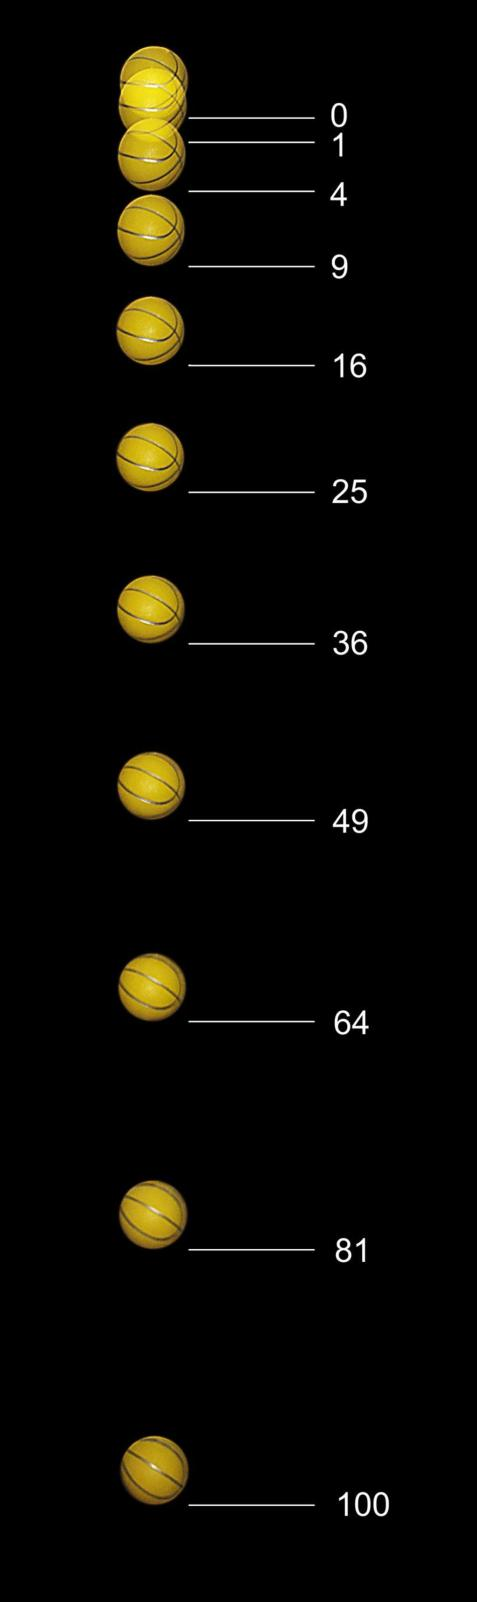
\includegraphics[height=5cm]{chronophoto_chute_libre.jpg}
  \caption{Chronophotographie d'un tir vertical ou d'une chute libre. La vitesse verticale n'étant pas constante, l'écart entre deux positions varie pour chaque prise de vue.}
  \label{chronophoto_chute_libre}
\end{figure}

\newpage

Pour résumer :\\
\begin{tabularx}{\linewidth}{m{.1\linewidth} X X X}
  \hline
                               & Ascension                                                & Descente                                                                        \\
  \hline
  \rotatebox{90}{Position}     & La position augmente mais de moins en moins vite.        & La position diminue de plus en plus vite.                                       \\[1.8cm]
  \hline
  \rotatebox{90}{Vitesse}      & La vitesse est positive, mais elle diminue linéairement. & La vitesse est négative et sa valeur augmente linéairement (en valeur absolue). \\[1.8cm]
  \hline
  \rotatebox{90}{Accélération} & L'accélération est constante et dirigée vers le bas.                                                                                       \\[1.8cm]
  \hline \hline
\end{tabularx}

\begin{figure}[!ht]
  \centering
  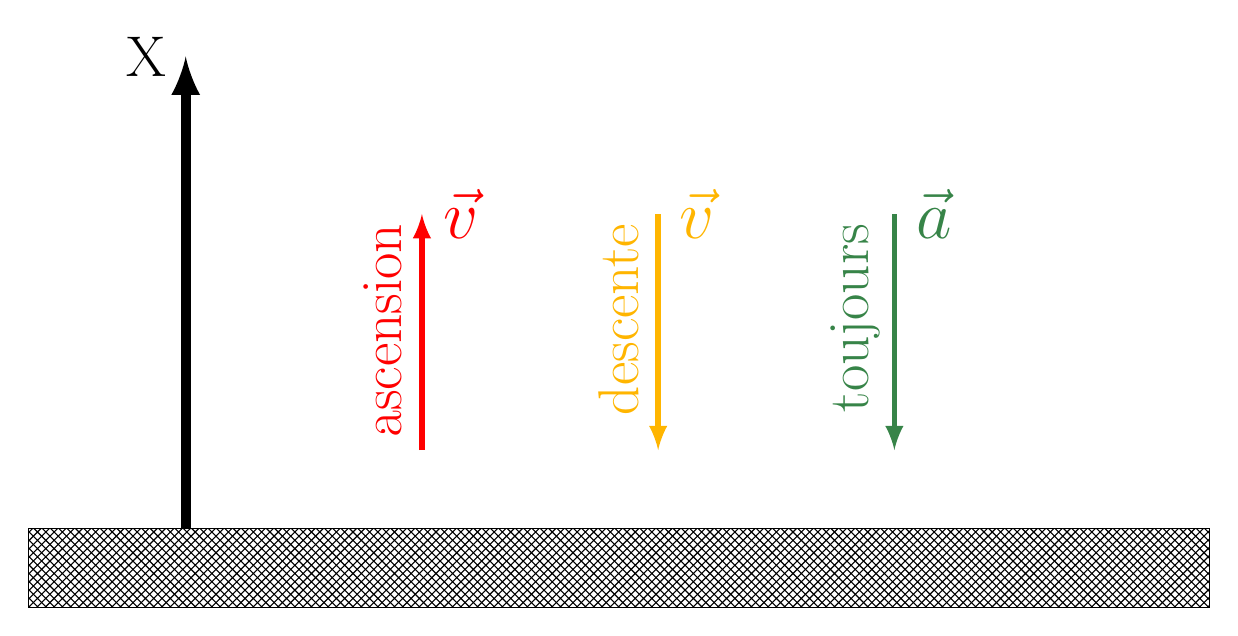
\begin{tikzpicture}[>=latex]
\usetikzlibrary[patterns]
\definecolor{jaune}{HTML}{ffb500}
\definecolor{rouge}{HTML}{ff0000}
\definecolor{vert}{HTML}{378448}

\filldraw [pattern=crosshatch](0,0) rectangle (15,1); %le rectangle du rail
\draw[->,line width=1.3mm](2,1)-- (2,7);%l'axe X
\node at (1.5,7) {\huge X};

\node [color=rouge,rotate=90,anchor=east] at (4.5,5) {\huge ascension};
\draw [->,line width=.7mm,color=rouge](5,2)-- (5,5);
\node [color=rouge] at (5.5,5) {\Huge $\vec{v}$};

\node [color=jaune,rotate=90,anchor=east] at (7.5,5) {\huge descente};
\draw [<-,line width=.7mm,color=jaune](8,2)-- (8,5);
\node [color=jaune]at (8.5,5) {\Huge $\vec{v}$};

\node [color=vert,rotate=90,anchor=east] at (10.5,5) {\huge toujours};
\draw [<-,line width=.7mm,color=vert](11,2)-- (11,5);
\node [color=vert] at (11.5,5){\Huge $\vec{a}$};




\end{tikzpicture} 

  \caption{Sens des vecteurs vitesse et accélération dans un tir vertical.}
  \label{vecteurs_tir_vertical}
\end{figure}

\newpage

\section{Graphiques}
Le tir vertical étant un MRUA, le graphique de la position sera une parabole, celui de la vitesse une droite et celui de l'accélération une constante.
\begin{tabularx}{\linewidth}{m{.1\linewidth} X X X}
  \hline
                               & Ascension & Descente \\
  \hline
  \rotatebox{90}{Position}     &           &          \\[4cm]
  \hline
  \rotatebox{90}{Vitesse}      &           &          \\[4cm]
  \hline
  \rotatebox{90}{Accélération} &           &          \\[4cm]
  \hline \hline
\end{tabularx}

\newpage

\section{Considérations mathématiques}
Lorsqu'un objet est lancé vers le haut, il existe une hauteur maximale qu'il ne dépasse pas. Par contre, tous les points situés en dessous de cette hauteur maximale sont atteint deux fois : durant l'ascension et durant la descente.
\begin{itemize}[label=\textbullet]

  \item Dans le cadre d'une application numérique sur le tir vertical, une question dans laquelle il faut trouver à quel moment le mobile passe par un point situé au-delà de la hauteur maximale, impliqueront la résolution d'une équation du deuxième degré avec un delta négatif. Il n'y a donc pas de solution à cette équation, car le mobile ne passe à aucun moment par un point plus haut que la hauteur maximale.
  \item Une question dans laquelle il faut trouver à quel moment le mobile passe par un point situé entre le sol et la hauteur maximale impliquera la résolution d'un système d'équation avec un delta positif. Il y aura donc deux valeurs de temps possibles : une à l'ascension et une autre à la descente.
  \item Le seul point qui est atteint une et une seule fois et celui correspondant à la hauteur maximale. Cela impliquera la résolution d'une équation avec un delta nul.
\end{itemize}

\newpage

\begin{figure}[!ht]
  \centering
   \begin{tikzpicture}[>=latex,scale=0.9]
            \tkzInit[xmax=20,ymax=20,xstep=2,ystep=2]
            \tkzGrid[]
            \tkzDrawX[label={$Temps\unit{[s]}$},below left=25pt]
            \tkzDrawY[label={$Position\unit{\unit{[m]}}$},right=5pt]
            \tkzAxeXY[label={}] %This macro combines the four macros: \tkzDrawX\tkzDrawY \tkzLabelX\tkzLabelY
            \tkzFct[domain =0:20,ultra thick,color=ForestGreen]{-0.1*(\x**2)+2*\x} %
            \tkzDefPoints{0/10/A,20/10/B}
            \tkzDefPoints{10/2/C,4/6/D,16/6/E}
            \tkzDrawSegment[->,gray](C,D)
            \tkzDrawSegment[->,gray](C,E)
            \tkzDrawSegment[color=red,ultra thick](A,B)
            \tkzText[draw, color=black,fill=lightgray,text width=7cm](10,16){Les points situés au-delà de la hauteur maximale ne sont jamais atteints}
            \tkzText[draw, color=black,fill=lightgray,text width=5cm](10,2){Les points situés en-dessous de la hauteur maximale sont atteints deux fois}

          \end{tikzpicture}

  \caption{Position en fonction du temps dans un tir vertical.}
  \label{position_tir_vertical}
\end{figure}

\newpage

\section{Exercices}
\begin{exercise}
  Un objet est lancé vers le haut avec une vitesse initiale de \(4\unit{[m/s]}\).
  \begin{enumerate}[label=\alph*)]
    \item Quelle est sa position après \(0,3\unit{[s]}\) ?
    \item Quelle est sa vitesse après \(0,5\unit{[s]}\) ?
    \item Que s'est-il passé entre ces deux instants ?
  \end{enumerate}
\end{exercise}

\begin{exercise}
  Un objet est lancé vers le haut avec une vitesse de \(2\unit{[m/s]}\).
  \begin{enumerate}[label=\alph*)]
    \item Quelle est sa vitesse lorsqu'il arrive au sommet de sa course ?
    \item À quel moment arrive-t-il au sommet de sa course ?
    \item Quelle est sa position à ce moment, c'est-à-dire quelle est la hauteur maximale atteinte par l'objet ?
  \end{enumerate}
\end{exercise}

\begin{exercise}
  Un objet est lancé vers le haut avec une vitesse de \(10 \unit{[m/s]}\).
  \begin{enumerate}[label=\alph*)]
    \item À quels moments atteint-il la hauteur de \(4\unit{[m]}\) ?
    \item À quel moment atteint-il la hauteur de \(200\unit{[m]}\) ?
    \item À quel moment atteint-il sa hauteur maximale ?
  \end{enumerate}
\end{exercise}

\begin{exercise}
  Un objet est lancé verticalement vers le haut avec une vitesse initiale de \(5[m \cdot s^{-1}]\) depuis le haut d'un immeuble de \(16\unit{[m]}\) de haut. L'objet va s'élever puis retomber au pied de l'immeuble.
  \begin{enumerate}[label=\alph*)]
    \item        Quelle est sa vitesse d'impact ?
    \item       Combien de temps dure le parcours de l'objet entre le moment où il est lancé vers le haut et celui où il touche le sol ?
  \end{enumerate}
\end{exercise}

\begin{exercise}
  Un objet tombe librement depuis une hauteur de \(75\unit{[m]}\). Lorsqu'il arrive à \(25 \unit{[m]}\) du sol, un deuxième objet est lancé vers le bas depuis la hauteur de \(75\unit{[m]}\). Quelle doit être la vitesse initiale du deuxième objet pour qu'il touche le sol en même temps que le premier ?
\end{exercise}

\begin{exercise}
  \qrcode{https://www.vf-bxl-moodle.be/mod/quiz/view.php?id=1354}
\end{exercise}